% Tamanho fonte | tamanho da página | tipo de documento
\documentclass[12pt]{article}


\usepackage[portuguese]{babel}
\usepackage[utf8]{inputenc}
\usepackage[T1]{fontenc}
\usepackage{graphicx}
\usepackage{mathtools}

\usepackage{hyperref}

\begin{document}

\begin{titlepage}

\newcommand{\HRule}{\rule{\linewidth}{0.5mm}} 

\center
 
%----------------------------------------------------------------------------------------
%	SEÇÃO CAPA
%----------------------------------------------------------------------------------------
\textsc{\LARGE Universidade de Évora}\\[1.5cm]
\begin{figure}[ht!]
\centering

\includegraphics[width=50mm]{UE.png}
\label{overflow}
\end{figure}
\indent \indent
\textsc{\Large Engenharia Informática}\\[0.5cm]
\textsc{\large Teoria da Informação}\\[0.5cm]

%----------------------------------------------------------------------------------------
%	SEÇÃO TÍTULO
%----------------------------------------------------------------------------------------

\HRule \\[0.4cm]
{ \huge \bfseries Trabalho Prático}\\[0.4cm] % Título do documento
\HRule \\[1.5cm]
 
%----------------------------------------------------------------------------------------
%	SEÇÃO AUTOR
%----------------------------------------------------------------------------------------

\begin{minipage}{0.4\textwidth}
\begin{flushleft} \large
\emph{Discente:}\\
Marcelo \textsc{Bábau} - 30372
José \textsc{Medeiro} - 31174
\end{flushleft}
\end{minipage}
\begin{minipage}{0.4\textwidth}
\begin{flushright} \large
\emph{Docente:} \\
Luis \textsc{Rato} \\  
\end{flushright}
\end{minipage}\\[4cm]

%----------------------------------------------------------------------------------------
%	SEÇÃO DATA	
%----------------------------------------------------------------------------------------

{\large \today}\\[3cm] % Date, change the \today to a set date if you want to be precise

\vfill % Fill the rest of the page with whitespace

\end{titlepage}

\tableofcontents

\newpage

%-------------------------------------------------------------------q---------------------
%	SEÇÃO 1
%----------------------------------------------------------------------------------------
\section{Introdução}
\indent \indent No âmbito da disciplina de Teoria da Informação foi proposto o desnvolvimento de uma amplicação de técnicas de compressão a uma sequência de ADN(sequências de pares base), que tem um alfabeto com 4 símbolos: "A", "C", "T", "G". Para tal implementámos um sistema para a transmissão de informação de uma fonte para um receptor através de um canal ruidoso. \newline
\indent Iremos utilizar um codificador e um descodificador, ligados à fonte e ao canal. O codificador vai consistir em compressão e codificação de dados. Na compressão de dados calculam-se as probabilidades de cada caractere, utilizando a compressão com Shannon-Fano-Elias.
\newline
\indent
Na descodificação fazemos o oposto da codificação e corrigimos os erros, se existirem.
\newpage


%----------------------------------------------------------------------------------------
%	SEÇÃO 2
%----------------------------------------------------------------------------------------
\section{Desenvolvimento do Programa}
\indent \indent Durante a realização deste trabalho, foi necessário modelar a fonte: Alfabeto, suas probabilidades, cadeia de Markov.
Foi também necessário, modelar o canal: probabilidades de transição.
\newline
\newline
\subsection{Modelo probabilístico da fonte} 
\subsubsection{Cálculo das probabilidades}
\indent\indent Alfabeto: "A","C","G","T".
\newline
\newline
\indent $P(x=A)=\frac{2374}{11008}=0.2157
\newline
\newline\indent P(x=C)=\frac{2874}{11008}=0.2611 
\newline
\newline\indent P(x=G)=\frac{3088}{11008}=0.2805 
\newline
\newline\indent P(x=T)=\frac{2672}{11008}=0.2427
$
\newline
\subsubsection{Cálculo da Entropia}
\indent\indent Entropia da fonte:
\newline
\indent $H(x)=-\sum{p(x)\log(p(x))}
\newline 
\newline\indent H(x)=-[(0.2157\log(0.2157))+(0.2611\log(0.2611))+(0.2805\log(0.2805))+(0.2427\log(0.2427))]=1.9934  bits
$
\newpage
\subsubsection{Compressão de dados Shannon-Fano-Elias}
\begin{figure}[ht!]
\centering
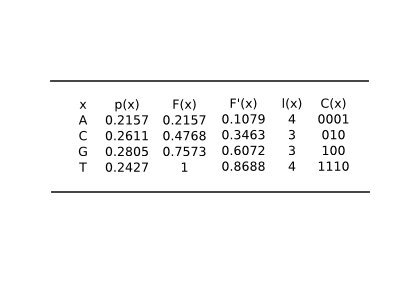
\includegraphics[width=100mm]{SFE.png}
\caption{Compressão de dados Shannon-Fano-Elias}
\label{overflow}
\end{figure}
\newpage
\subsection{Modelo probabilístico do canal}
\indent\indent O canal que nos foi proposto, é um Canal em Z, ou seja um canal assimétrico.
\begin{figure}[ht!]
\centering
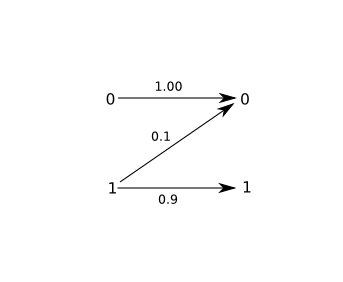
\includegraphics[width=50mm]{CanalZ.png}
\caption{Canal Assimétrico}
\label{overflow}
\end{figure}
\newpage
\subsection{Codificador}
\indent Para criar o codificador(Code.java)tivemos de inicializar dois objetos fundamentais para a codificação. As classes ShannonFanoElias.java e Hamming.java, são utilizadas respetivamente para nos gerar um código Shannon-Fano-Elias para comprimir a mensagem e depois utilizamos a codificação de Hamming(7,4) para conseguirmos detectar os erros na descodificação.
\newline
\newline
\newline
\subsection{Descodificador}
\indent\indent O descodificador(Decode.java) é o processo inverso do codificador. Depois de recebermos o input, que é a mensagem codificada, voltamos a usar classes ShannonFanoElias.java e Hamming.java, mas por ordem contrária e a função de descodificar. Em primeiro lugar, detectam-se os erros utilizando a classe Hamming.java e retiram-se os bits de paridade. De seguida, utilizando a classe ShannonFanoElias.java, fazemos a conversão dos códigos(0001,010,100,1110) de volta para os símbolos("A","C","G","T").
\newpage
\section{Conclusão}
\indent \indent Neste trabalho, achamos que não tivemos a totalidade dos objetivos cumpridos, pois tivemos alguns problemas no canal, e o nosso ficheiro com a codificação com os caracteres "0" e "1", não foi gerado como um ficheiro binário, o que nos leva a pensar que o número de erros seja maior.



\end{document} 